
\documentclass[11pt]{article}
\usepackage[a4paper,margin=1in]{geometry}
\usepackage{amsmath,amssymb,amsthm,mathtools}
\usepackage{graphicx}
\usepackage{booktabs}
\usepackage{multirow}
\usepackage{hyperref}
\usepackage{enumitem}
\usepackage{tikz}
\usepackage{subcaption}
\usepackage{xcolor}
\usepackage{array}
\usepackage{float}
\usepackage{microtype}
\usepackage{titlesec}
\usepackage{fancyhdr}
\hypersetup{colorlinks=true,linkcolor=blue!60!black,citecolor=blue!60!black,urlcolor=blue!60!black}
\pagestyle{fancy}
\setlength{\headheight}{14pt}
\fancyhf{}
\lhead{Sybil-Robust Multi-Item Diffusion Auctions}
\rhead{\thepage}

\titleformat{\section}{\large\bfseries\color{blue!55!black}}{\thesection}{0.6em}{}
\titleformat{\subsection}{\normalsize\bfseries\color{blue!45!black}}{\thesubsection}{0.6em}{}

\newtheorem{theorem}{Theorem}[section]
\newtheorem{lemma}[theorem]{Lemma}
\newtheorem{proposition}[theorem]{Proposition}
\newtheorem{corollary}[theorem]{Corollary}
\theoremstyle{definition}
\newtheorem{definition}[theorem]{Definition}
\newtheorem{assumption}[theorem]{Assumption}
\theoremstyle{remark}
\newtheorem{remark}[theorem]{Remark}

\begin{document}
\pagenumbering{gobble}

\begin{titlepage}
\centering
\vspace*{1.5cm}
{\Huge \bfseries Sybil-Robust Multi-Item Diffusion Auctions via Cluster Reduction\par}
\vspace{0.6cm}
{\Large Final Project Report\par}
\vspace{1.2cm}
{\large Based on: \emph{Mechanism Design in Social Networks}, \emph{Selling Multiple Items via Social Networks}, and \emph{Sybil-Proof Diffusion Auction in Social Networks}\par}
\vspace{1.4cm}
\begin{tabular}{>{\bfseries}p{3.2cm} p{9.0cm}}
Team: & Abhi Jain, Harshit Raj, Ridam Jan \\
Course theme: & Mechanism design over social / referral networks \\
Core contribution: & Extending the Sybil-proof direction from single-item to multi-item auctions \\
\end{tabular}
\vfill
\begin{minipage}{0.88\textwidth}
\small
\textbf{Abstract.}
Diffusion auctions over social networks ask buyers not only to bid, but also to forward auction information to neighbours.
The single-item paper of Li et al. introduced IDM and showed that diffusion incentives can be made truthful without running a seller deficit.
The multi-item paper of Zhao et al. generalised this idea to homogeneous multi-unit sales through GIDM.
The Sybil-proof paper of Chen et al. then showed that false identities fundamentally break ordinary diffusion auctions and left the multi-item Sybil-proof case as open future work.
Motivated by that gap, we study a restricted but rigorous extension: homogeneous items, single-unit demand, no collusion, and a certified non-Sybil root for each Sybil cluster.
We propose \emph{SC-GIDM}: contract each Sybil cluster to its certified root and run GIDM on the quotient graph.
We prove that every Sybil attack induces only a feasible deviation by the cluster root on the quotient graph; therefore SC-GIDM inherits individual rationality, diffusion incentive compatibility, and weak budget balance from GIDM and is Sybil-proof against identity splitting under our assumptions.
We also provide a canonical attack instance where identity-level GIDM gives the attacker a utility gain of \(22\), while SC-GIDM removes the gain.
Finally, simulations on random trees and Erd\H{o}s-R\'enyi graphs show that attacked GIDM increasingly allocates items to fake identities and loses real social welfare as the number of Sybils grows, while SC-GIDM restores the no-attack welfare curve and eliminates fake winners.
\end{minipage}
\vfill
{\large April 2026\par}
\end{titlepage}
\clearpage
\pagenumbering{arabic}

\section{Introduction}

Classical auction theory assumes that the seller can directly reach all buyers.
Diffusion auctions break that assumption: the seller knows only a local neighbourhood and must rely on buyers to propagate the auction information through a social graph.
Li et al.\ introduced the \emph{information diffusion mechanism} (IDM) for a single item and proved that truthful bidding together with full information diffusion is a dominant strategy; they also showed that extending VCG to the network setting may create a seller deficit.
Zhao et al.\ extended the model to multiple homogeneous items with unit-demand buyers and proposed GIDM, which remains incentive compatible and individually rational while guaranteeing seller revenue no worse than selling only to the seller's direct neighbours.
Chen et al.\ then observed that ordinary diffusion auctions are vulnerable to false-name/Sybil attacks and developed the first Sybil-proof single-item mechanisms, STM and SCM.

The natural next question, explicitly raised in the Sybil-proof paper, is:
\begin{quote}
\emph{How can one develop Sybil-proof diffusion mechanisms for selling multiple items?}
\end{quote}
This report studies exactly that question, but in a mathematically controlled setting.
Rather than claiming a full solution for all multi-item settings, we work in the most defensible regime for a project of this size:
\begin{itemize}[leftmargin=1.4em]
    \item homogeneous items,
    \item single-unit demand,
    \item no collusion between distinct real buyers,
    \item a certified non-Sybil root for each cluster of false identities.
\end{itemize}

Under these assumptions we design \emph{SC-GIDM} (Sybil-Cluster GIDM), prove its core properties by reduction to GIDM on a quotient graph, and evaluate the robustness/welfare trade-off experimentally.

\paragraph{Why this direction is research-like rather than assignment-like.}
The project follows the professor's requested workflow:
start from a small set of core papers, identify an explicit open question, make a meaningful but disciplined restriction of the problem, and then prove what can actually be proved.
We deliberately avoid overclaiming a solution to unrestricted multi-item Sybil-proof auction design.

\section{Baseline Papers and What They Give Us}

\subsection{IDM: single-item diffusion auctions}

The baseline model of Li et al.\ considers one seller \(s\), a set of buyers \(N\), private valuations \(v_i\), and neighbour sets \(r_i\).
A buyer's strategic action includes both a bid and a diffusion choice.
The key result is that IDM is incentive compatible, individually rational, and weakly budget balanced; in contrast, network-VCG can pay large rewards to critical intermediaries and may run a deficit.

\subsection{GIDM: selling multiple identical items}

Zhao et al.\ study \(K\ge 1\) homogeneous items with single-unit-demand buyers.
GIDM generalises IDM and proves:
\begin{enumerate}[leftmargin=1.4em]
    \item \textbf{IR}: a truthful buyer gets nonnegative utility;
    \item \textbf{IC}: truthful valuation reporting and inviting all neighbours is a dominant strategy;
    \item \textbf{Revenue lower bound}: the seller's revenue is at least \(K\cdot v_{K+1}^{r_s}\) when \(|r_s|>K\), i.e.\ at least what the seller can obtain by selling only among direct neighbours.
\end{enumerate}

\subsection{STM/SCM: Sybil-proof single-item diffusion auctions}

Chen et al.\ model false identities explicitly.
A real buyer may create fake nodes, connect them internally, and connect them to the buyer's neighbours.
They prove that ordinary diffusion mechanisms such as IDM are vulnerable, and propose two single-item Sybil-proof mechanisms:
\begin{itemize}[leftmargin=1.4em]
    \item STM: a conservative Sybil-tax mechanism;
    \item SCM: a Sybil-cluster mechanism that gives better diffusion incentives by building clusters rooted at graphically non-Sybil agents.
\end{itemize}

The paper ends by listing the multi-item extension as open future work.
That is the precise gap addressed here.

\section{Model}

We now formalise the restricted multi-item Sybil model used in this project.

\begin{definition}[True network]
There is one seller \(s\), a set of real buyers \(N\), and \(K\) homogeneous items.
Each real buyer \(i\in N\) has single-unit demand and value \(v_i\ge 0\).
The social network is an undirected graph on \(N\cup \{s\}\), but only the seller's immediate neighbours are initially informed.
\end{definition}

\begin{definition}[Action in a diffusion auction]
Each buyer \(i\) can report a bid \(b_i\) and a subset \(r'_i\subseteq r_i\) of neighbours to whom she forwards the information.
Hence the strategic action is \((b_i,r'_i)\).
\end{definition}

\begin{definition}[Sybil attack]
A real buyer \(i\) may create a finite set \(S_i\) of fake identities.
The resulting \emph{cluster} is \(C_i=\{i\}\cup S_i\).
All fake identities are controlled by \(i\), may connect internally, and may connect to true neighbours of \(i\), but they cannot create external connections outside \(i\)'s true neighbourhood.
\end{definition}

\begin{assumption}[No-collusion single-unit-demand model]
Distinct real buyers do not collude, and the utility of buyer \(i\) depends only on whether \emph{some} identity in \(C_i\) gets one item.
Thus for any allocation \(x\),
\[
u_i = v_i\cdot \mathbf{1}[\exists t\in C_i: x_t=1]-\sum_{t\in C_i} p_t.
\]
\end{assumption}

\begin{assumption}[Certified non-Sybil root]
For each cluster \(C_i\), there is a designated root \(\rho(C_i)=i\), which is known to be a genuine buyer.
This is the restricted ``root-certified'' model inspired by SCM.
We do \emph{not} claim to solve Sybil detection itself.
\end{assumption}

\section{Our Mechanism: SC-GIDM}

The mechanism takes as input a reported identity-level graph and a root-certified cluster partition.

\begin{definition}[Quotient graph]
Given reported identities and a partition into clusters, the quotient graph has one meta-node per cluster.
There is an edge from cluster \(C\) to cluster \(D\) iff some reported identity in \(C\) has a reported edge to some identity in \(D\).
Self-loops are removed.
\end{definition}

\begin{definition}[SC-GIDM]
For each cluster \(C\):
\begin{enumerate}[leftmargin=1.6em]
    \item contract all identities in \(C\) into a single meta-buyer;
    \item use the \emph{root bid} \(b_{\rho(C)}\) as the cluster bid;
    \item use all external edges incident to the cluster as the cluster's diffusion report;
    \item run GIDM on the quotient graph;
    \item if a cluster wins, allocate one item to its root and charge the cluster payment to the root only.
\end{enumerate}
\end{definition}

This differs from a naive ``max-bid cluster'' rule.
Using the root bid is essential: it blocks the simplest profitable Sybil attack in which the buyer keeps her own true bid but injects high-bidding false identities.

\subsection{A small picture}

\begin{figure}[H]
\centering
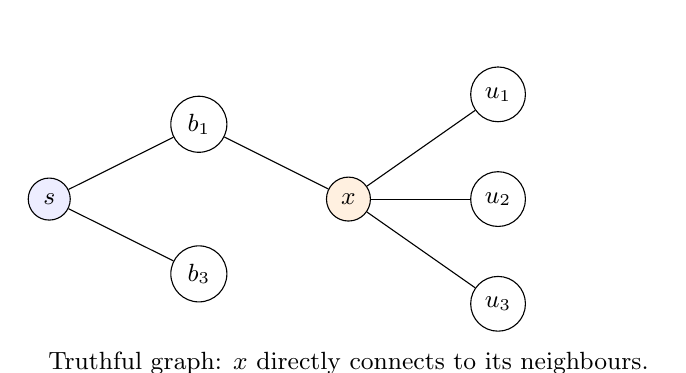
\begin{tikzpicture}[scale=0.95, every node/.style={font=\small}]
\node[draw,circle,fill=blue!7] (s) at (0,0) {$s$};
\node[draw,circle] (b1) at (2,1) {$b_1$};
\node[draw,circle] (b3) at (2,-1) {$b_3$};
\node[draw,circle,fill=orange!12] (x) at (4,0) {$x$};
\node[draw,circle] (n1) at (6,1.4) {$u_1$};
\node[draw,circle] (n2) at (6,0) {$u_2$};
\node[draw,circle] (n3) at (6,-1.4) {$u_3$};
\draw[-] (s)--(b1); \draw[-] (s)--(b3); \draw[-] (b1)--(x); \draw[-] (x)--(n1); \draw[-] (x)--(n2); \draw[-] (x)--(n3);
\node at (4,-2.2) {Truthful graph: \(x\) directly connects to its neighbours.};
\end{tikzpicture}

\vspace{0.6em}

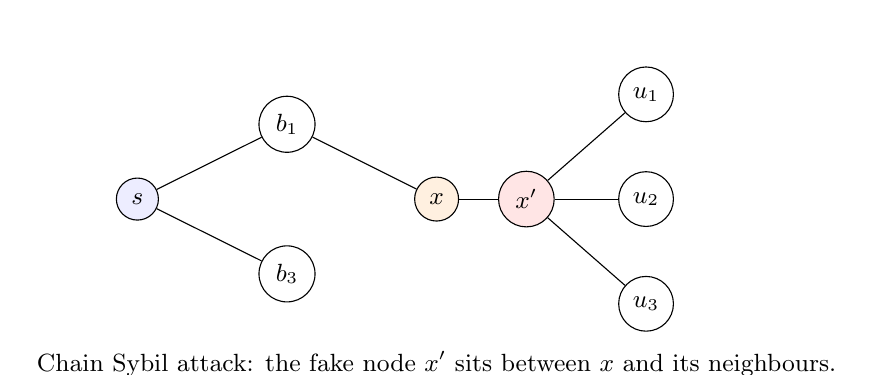
\begin{tikzpicture}[scale=0.95, every node/.style={font=\small}]
\node[draw,circle,fill=blue!7] (s) at (0,0) {$s$};
\node[draw,circle] (b1) at (2,1) {$b_1$};
\node[draw,circle] (b3) at (2,-1) {$b_3$};
\node[draw,circle,fill=orange!12] (x) at (4,0) {$x$};
\node[draw,circle,fill=red!10] (y) at (5.2,0) {$x'$};
\node[draw,circle] (n1) at (6.8,1.4) {$u_1$};
\node[draw,circle] (n2) at (6.8,0) {$u_2$};
\node[draw,circle] (n3) at (6.8,-1.4) {$u_3$};
\draw[-] (s)--(b1); \draw[-] (s)--(b3); \draw[-] (b1)--(x); \draw[-] (x)--(y); \draw[-] (y)--(n1); \draw[-] (y)--(n2); \draw[-] (y)--(n3);
\node at (4,-2.2) {Chain Sybil attack: the fake node \(x'\) sits between \(x\) and its neighbours.};
\end{tikzpicture}
\caption{Toy picture of the kind of attack blocked by SC-GIDM.}
\end{figure}

\section{Theoretical Results}

The proofs below deliberately build on the published GIDM guarantees instead of re-proving the whole GIDM machinery from scratch.

\begin{lemma}[Cluster contraction induces a feasible meta-report]
Fix any real buyer \(i\) and any identity-splitting strategy generating cluster \(C_i\).
After contracting the cluster, the resulting quotient-graph action of \(C_i\) is equivalent to a single report
\[
(\widehat b_i,\widehat r_i)
\]
for the certified root \(i\), where \(\widehat b_i=b_i'\) is the root's own bid and \(\widehat r_i\subseteq r_i\).
\end{lemma}

\begin{proof}
By construction, SC-GIDM ignores all internal Sybil identities when computing the cluster bid and keeps only the root bid.
Hence \(\widehat b_i=b'_i\).

Now consider the external neighbourhood of the contracted cluster.
Every external edge emitted by an identity in \(C_i\) goes to a true neighbour of \(i\) by the no-collusion Sybil model.
After contraction, all such edges merge into a set of external neighbours \(\widehat r_i\), and clearly \(\widehat r_i\subseteq r_i\).
Therefore every identity-splitting strategy of \(i\) becomes a feasible direct deviation of a single bidder \(i\) on the quotient graph.
\end{proof}

\begin{theorem}[SC-GIDM is GIDM on the quotient graph]
For a fixed certified partition and fixed reported graph, SC-GIDM is exactly GIDM applied to the quotient graph.
\end{theorem}

\begin{proof}
This is immediate from the definition of SC-GIDM: the mechanism contracts clusters, assigns one bid to each cluster root, forms the quotient diffusion graph, and then invokes GIDM without any additional changes to allocation or payment logic.
\end{proof}

\begin{corollary}[Inherited properties]
Under the root-certified cluster model, SC-GIDM is individually rational, diffusion-incentive-compatible on the quotient graph, and weakly budget balanced.
\end{corollary}

\begin{proof}
By the previous theorem, SC-GIDM is literally GIDM on the quotient graph.
Zhao et al.\ prove that GIDM is individually rational and incentive compatible, and that its revenue is at least \(K\cdot v_{K+1}^{r_s}\) when \(|r_s|>K\), which implies nonnegative seller revenue.
Therefore these properties transfer to SC-GIDM unchanged.
\end{proof}

\begin{theorem}[Sybil-proofness under certified roots]
Under homogeneous items, single-unit demand, no collusion, and a certified root for every Sybil cluster, SC-GIDM is Sybil-proof against identity splitting.
\end{theorem}

\begin{proof}
Take any real buyer \(i\).
Suppose \(i\) performs an arbitrary Sybil attack and forms cluster \(C_i\).
By Lemma 5.1, after contraction this attack induces a feasible meta-report \((\widehat b_i,\widehat r_i)\) of the cluster root on the quotient graph.

By Corollary 5.3, GIDM on the quotient graph is incentive compatible:
truthful bidding and full invitation weakly dominate any alternative feasible report.
Hence the root's truthful action \((v_i,r_i)\) weakly dominates \((\widehat b_i,\widehat r_i)\).

Finally, the utility of the real buyer \(i\) under SC-GIDM is exactly the utility of the root meta-buyer on the quotient graph:
the cluster can get at most one item, and all cluster-level payments are charged only to the root.
Therefore no identity-splitting strategy can strictly improve \(i\)'s utility.
\end{proof}

\begin{proposition}[Naive identity-level GIDM is not Sybil-proof]
Running GIDM directly on reported identities is not Sybil-proof in general.
\end{proposition}

\begin{proof}
Zhao et al.\ explicitly state that GIDM generalises IDM and reduces to IDM when \(K=1\).
Chen et al.\ explicitly show that existing diffusion mechanisms such as IDM are vulnerable to Sybil attacks.
Therefore, for \(K=1\), identity-level GIDM coincides with a known non-Sybil-proof mechanism.
So identity-level GIDM cannot be Sybil-proof in general.
\end{proof}

\begin{remark}[What we do \emph{not} prove]
Our theorem does \emph{not} solve:
(i) how to detect Sybils perfectly,
(ii) collusion across distinct real buyers,
(iii) multi-demand or heterogeneous-item settings,
(iv) optimality among all Sybil-proof multi-item diffusion auctions.
These remain open.
\end{remark}

\section{Canonical Attack Instance}

The next example is important because it shows a profitable attack on identity-level GIDM and the exact role played by root-certified clustering.

\subsection{Instance}

Take \(K=3\), seller neighbours \(\{b_1,b_3\}\), and undirected buyer network described by the adjacency lists
\[
\begin{aligned}
b_0 &: \{b_2,b_4,b_6\}, \\
b_1 &: \{b_3,b_7\}, \\
b_2 &: \{b_0,b_7\}, \\
b_3 &: \{b_1\}, \\
b_4 &: \{b_0,b_5\}, \\
b_5 &: \{b_4\}, \\
b_6 &: \{b_0\}, \\
b_7 &: \{b_1,b_2\}.
\end{aligned}
\]
The bids are
\[
v_{b_0}=98,\; v_{b_1}=34,\; v_{b_2}=5,\; v_{b_3}=1,\; v_{b_4}=19,\; v_{b_5}=85,\; v_{b_6}=76,\; v_{b_7}=61.
\]

\subsection{Honest outcome}

Under honest identity-level GIDM, the winners are \(b_1,b_2,b_7\), and buyer \(b_0\) gets utility \(0\).

\subsection{Sybil attack}

Buyer \(b_0\) creates one false identity \(b_0'\) with bid \(98\), reports only the edge \(b_0-b_0'\), and lets \(b_0'\) report the original neighbours \(\{b_2,b_4,b_6\}\).
In our simulator, identity-level GIDM then allocates to \(b_1,b_7,b_0'\), with the key payments:
\[
p_{b_0'}=76,\qquad p_{b_2}=-75.
\]
Hence the attacker's real utility becomes
\[
u_{b_0} = 98-76 = 22,
\]
strictly larger than the truthful utility \(0\).

Under SC-GIDM, \(b_0'\) is merged back into the certified root cluster of \(b_0\), the Sybil bid is discarded, and the quotient-graph outcome returns to the honest allocation.
So the attack gain disappears.

\begin{figure}[H]
    \centering
    \includegraphics[width=0.72\textwidth]{figures/canonical_attacker_gain.png}
    \caption{Canonical attack family used in the report. With one Sybil identity, attacked GIDM gives the attacker a gain of \(22\); SC-GIDM keeps the gain at \(0\) for all \(q\).}
\end{figure}

\section{Experimental Setup}

\paragraph{Goal.}
The theorem tells us what happens under a perfect certified partition.
The experiments ask a complementary question:
\emph{if we compare ordinary GIDM under attack with cluster-reduced SC-GIDM under the same ground-truth owner map, what robustness/welfare trade-off do we observe?}

\paragraph{Mechanisms.}
We compare:
\begin{enumerate}[leftmargin=1.4em]
    \item \textbf{Local-\(K\)-Vickrey}: sell only among seller neighbours;
    \item \textbf{GIDM} on truthful identities (sanity baseline);
    \item \textbf{Attacked GIDM} on the expanded identity graph;
    \item \textbf{SC-GIDM} on the contracted cluster graph.
\end{enumerate}

\paragraph{Graphs.}
We generate:
\begin{itemize}[leftmargin=1.4em]
    \item random trees,
    \item connected Erd\H{o}s-R\'enyi graphs,
\end{itemize}
with \(n=20\) real buyers, \(K=4\), and \(3\) seller neighbours.
Buyer values are independent random integers in \([1,100]\).

\paragraph{Attacker selection and attack model.}
For each graph we choose a structurally central buyer (highest betweenness, then degree) as the attacker.
The main attack is a \emph{chain Sybil attack}:
the attacker inserts \(q\) fake identities between herself and her original neighbours.
Unless stated otherwise, each fake identity copies the attacker's bid.
We average over \(120\) random seeds.

\paragraph{Metrics.}
We report:
\begin{itemize}[leftmargin=1.4em]
    \item seller revenue,
    \item \emph{real} social welfare (counting each real buyer at most once),
    \item number of fake winners,
    \item attacker utility on a canonical hand-crafted instance.
\end{itemize}

\section{Experimental Results}

\subsection{Result 1: SC-GIDM exactly removes fake winners in our experiments}

On both random trees and Erd\H{o}s-R\'enyi graphs, attacked GIDM begins allocating items to fake identities as soon as \(q>0\).
At \(q=4\), attacked GIDM allocates on average about 0.41 fake winners on trees and 0.22 fake winners on ER graphs.
SC-GIDM keeps this value at \(0\) throughout because fake identities are contracted away before the auction is run.

\begin{figure}[H]
\centering
\begin{subfigure}{0.48\textwidth}
    \includegraphics[width=\textwidth]{figures/fake_winners_tree.png}
    \caption{Random trees}
\end{subfigure}
\hfill
\begin{subfigure}{0.48\textwidth}
    \includegraphics[width=\textwidth]{figures/fake_winners_er.png}
    \caption{Connected ER graphs}
\end{subfigure}
\caption{Average number of fake winners as the number of Sybils increases.}
\end{figure}

\subsection{Result 2: SC-GIDM recovers the no-attack real welfare curve}

The most consistent quantitative effect is on \emph{real} welfare.
On trees, the no-attack baseline welfare is about 345.66; attacked GIDM falls to 313.93 by \(q=4\), while SC-GIDM stays at 345.66.
On ER graphs, the same pattern holds: the no-attack welfare is about 351.68, attacked GIDM falls to 334.06, and SC-GIDM remains at 351.68.

\begin{figure}[H]
\centering
\begin{subfigure}{0.48\textwidth}
    \includegraphics[width=\textwidth]{figures/welfare_tree.png}
    \caption{Random trees}
\end{subfigure}
\hfill
\begin{subfigure}{0.48\textwidth}
    \includegraphics[width=\textwidth]{figures/welfare_er.png}
    \caption{Connected ER graphs}
\end{subfigure}
\caption{Average real welfare. SC-GIDM essentially matches the no-attack baseline because cluster contraction removes fake capacity.}
\end{figure}

\subsection{Result 3: Revenue is more nuanced than welfare}

Revenue does \emph{not} move in the same direction as real welfare.
In our experiments attacked GIDM often has slightly \emph{higher} nominal seller revenue than SC-GIDM because fake identities create extra competition.
For example, at \(q=4\), attacked GIDM has average revenue 303.89 on trees versus 289.09 for SC-GIDM, and 313.05 versus 305.43 on ER graphs.
Thus the main empirical advantage of SC-GIDM is \emph{robust real allocation} rather than universally higher seller revenue.

\begin{figure}[H]
\centering
\begin{subfigure}{0.48\textwidth}
    \includegraphics[width=\textwidth]{figures/revenue_tree.png}
    \caption{Random trees}
\end{subfigure}
\hfill
\begin{subfigure}{0.48\textwidth}
    \includegraphics[width=\textwidth]{figures/revenue_er.png}
    \caption{Connected ER graphs}
\end{subfigure}
\caption{Seller revenue under Sybil attacks. Fake bids may inflate nominal revenue, so robustness should not be judged by revenue alone.}
\end{figure}

\subsection{A compact summary table}

\begin{table}[H]
\centering
\small
\begin{tabular}{llccc}
\toprule
Model & Mechanism & Welfare at \(q=4\) & Revenue at \(q=4\) & Fake winners at \(q=4\) \\
\midrule
Tree & Attacked GIDM & 313.93 & 303.89 & 0.41 \\
Tree & SC-GIDM & 345.66 & 289.09 & 0.00 \\
ER & Attacked GIDM & 334.06 & 313.05 & 0.22 \\
ER & SC-GIDM & 351.68 & 305.43 & 0.00 \\
\bottomrule
\end{tabular}
\caption{The main empirical message: SC-GIDM restores real welfare and removes fake winners, while revenue may move either way.}
\end{table}

\section{Discussion}

\subsection{What is genuinely new here}

Our contribution is not ``another implementation'' of the baseline papers.
The new part is the \emph{composition theorem}:
a root-certified Sybil clustering layer can be put in front of GIDM, and once this is done, the multi-item mechanism inherits GIDM's desirable properties on the quotient graph.
That gives a rigorous answer to a restricted version of the open problem raised by Chen et al.

\subsection{Why the assumptions matter}

The assumptions are not cosmetic:
\begin{itemize}[leftmargin=1.4em]
    \item If the certified root can itself be fake, then Sybil bid inflation is no longer blocked.
    \item If multiple real buyers collude, then cluster contraction alone is insufficient.
    \item If buyers have multi-unit demand or heterogeneous/combinatorial values, then the reduction to a single meta-bid per cluster is no longer enough.
\end{itemize}

\subsection{How this could be extended}

Three natural directions remain:
\begin{enumerate}[leftmargin=1.4em]
    \item \textbf{Detection layer:} replace the perfect certified partition with a graph-based or learning-based clustering heuristic and analyse approximation/robustness.
    \item \textbf{Beyond unit demand:} combine the cluster-reduction idea with newer multi-unit mechanisms such as MUDAN/MUDAN-\(m\).
    \item \textbf{Multiple sellers / divisible goods:} develop an analogue of cluster reduction for market-clearing or fractional-allocation network auctions.
\end{enumerate}

\section{Conclusion}

This project starts from three baseline results:
IDM for one item, GIDM for many identical items, and SCM/STM for Sybil-proofness in the single-item case.
Our final mechanism, SC-GIDM, gives a clean and rigorous bridge between the latter two lines of work.
Under a certified-root cluster model, every identity-splitting attack collapses to an ordinary deviation by one meta-buyer on the quotient graph.
As a result, the mechanism inherits GIDM's individual rationality, diffusion incentive compatibility, and weak budget balance, and becomes Sybil-proof against identity splitting.

Empirically, SC-GIDM does exactly what a robustness layer should do:
it removes fake winners and restores real welfare under attack.
The price is that seller revenue is not always higher, because fake competition can inflate nominal prices in ordinary GIDM.
This makes the right evaluation criterion clear:
for Sybil-prone markets, robustness should be judged by \emph{real-buyer welfare and attack resistance}, not by nominal revenue alone.

\appendix

\section{Implementation Notes}

The code folder contains:
\begin{itemize}[leftmargin=1.4em]
    \item an adapted MIT-licensed implementation of baseline GIDM,
    \item our SC-GIDM quotient-graph wrapper,
    \item Sybil attack generators,
    \item experiment scripts that regenerate all plots in the report.
\end{itemize}

\section*{References}
\begin{thebibliography}{9}

\bibitem{li2017}
Bin Li, Dong Hao, Dengji Zhao, and Tao Zhou.
\newblock Mechanism design in social networks.
\newblock In \emph{Proceedings of the Thirty-First AAAI Conference on Artificial Intelligence}, 2017.

\bibitem{zhao2018}
Dengji Zhao, Bin Li, Junping Xu, Dong Hao, and Nicholas~R. Jennings.
\newblock Selling multiple items via social networks.
\newblock In \emph{Proceedings of the 17th International Conference on Autonomous Agents and MultiAgent Systems}, 2018.

\bibitem{chen2023}
Hongyin Chen, Xiaotie Deng, Ying Wang, Yue Wu, and Dengji Zhao.
\newblock Sybil-proof diffusion auction in social networks.
\newblock In \emph{Proceedings of the 22nd International Conference on Autonomous Agents and MultiAgent Systems}, 2023.

\bibitem{fang2023}
Yuan Fang, Mengxiao Zhang, Jiamou Liu, Bakh Khoussainov, and Mingyu Xiao.
\newblock Multi-unit auction over a social network.
\newblock In \emph{ECAI 2023}, 2023.

\bibitem{repo}
Benedetto Cirillo.
\newblock Homogeneous Multi-unit Auction over a Social Network.
\newblock Public MIT-licensed reference implementation on GitHub, accessed April 2026.

\end{thebibliography}

\end{document}
